% Srikar's section. Insert immediately before \end{document}.
% Results from the junction-area-consistent artifacts at commit 29d644c.
\clearpage
\section{Circuit-Level Validation: Parity Checker}
\label{sec:circuit}

\subsection{Aim}
This part extends the gate-level method to a complete circuit. The aim is
to estimate its static supply leakage by combining predictions for its
individual gates, and compare the estimate with a transistor-level SPICE
simulation of the complete circuit.

\subsection{Circuit construction}
The circuit checks eight data bits, $d_0,\ldots,d_7$, together with an
even-parity bit $p$. Its output is
\begin{equation}
e=d_0\oplus d_1\oplus\cdots\oplus d_7\oplus p.
\end{equation}
An output of 0 indicates valid even parity; an output of 1 indicates a
parity error. There are nine primary inputs and $2^9=512$ input vectors.
The vector order used throughout is $d_0,d_1,\ldots,d_7,p$.

The eight data bits are combined using a balanced XOR tree. Its output is
then XORed with the parity bit. Each of the eight XOR operations is built
from four NAND2 gates:
\begin{align}
t_1&=\operatorname{NAND}(a,b), &
t_2&=\operatorname{NAND}(a,t_1),\\
t_3&=\operatorname{NAND}(b,t_1), &
a\oplus b&=\operatorname{NAND}(t_2,t_3).
\end{align}
The complete circuit therefore contains 32 NAND2 gates and 128 transistors.
Each NAND2 uses the same topology and minimum transistor sizing as Part 3:
$W=L=22$\,nm. The device setup uses drain and source
areas $AD=AS=W(2L)$. The transistor netlist contains no ideal logic gates
and no added output load.

One ordered list of gate connections is used for both Boolean evaluation
and netlist generation. NAND inputs retain their order: input $a$ drives
the upper NMOS in the stack and input $b$ drives the lower NMOS. This matters
because states \texttt{01} and \texttt{10} need not have the same leakage.

\subsection{PVT conditions and SPICE reference}
The evaluation uses the same 200 PVT corners as Part 3. Each corner specifies
the supply voltage, temperature, and separate NMOS and PMOS process
parameters. Evaluating every input vector at every corner gives
$512\times200=102{,}400$ circuit cases. These are 200 distinct PVT draws,
each reused for all 512 vectors.

The reference leakage is the current drawn from the complete circuit's
shared supply, $I_{\mathrm{SPICE}}=-i(\texttt{vsupply})$. Current supplied by
the separate primary-input sources is excluded from this main definition.
The simulator records the supply current, primary-input currents, and all
32 NAND output voltages. A DC sweep enumerates the binary inputs using
sources that hold each input at exactly 0 or $V_{DD}$. The circuit itself
remains a transistor-level circuit. Independent operating-point simulations
provide a cross-check of this sweep method.

\subsection{Hierarchical estimate from the transistor models}
The circuit estimate reuses the Part 3 NAND2 predictions. At each corner,
a lookup table contains the four ordered NAND input states, giving
$4\times200=800$ entries. Each entry contains the gate's predicted supply
leakage and the signed gate currents at its two input pins. The supply
leakage uses the KCL method described in Section~\ref{sec:combine}.
For a NAND input pin, its current is the sum of the gate-terminal currents
of the PMOS and NMOS connected to that pin.

For each nine-bit input vector, Boolean evaluation determines the input
state of every NAND. The corresponding lookup entry is selected for each
gate and the contributions are combined. The circuit estimate does not
use node voltages from the complete-circuit SPICE simulation. However,
the isolated-gate lookup inherits the SPICE-recorded transistor voltages
used by Part 3; it is therefore a hierarchical approximation based on
characterised gates.

\subsection{Combining the gate contributions}
\paragraph{Plain gate sum (baseline).}
The prescribed hierarchical estimate adds the supply leakages of the
32 isolated NAND gates:
\begin{equation}
\widehat I_{\mathrm{plain}}=\sum_{j=1}^{32}\widehat I_{\mathrm{supply},j}.
\end{equation}
This baseline is retained in the comparison.

\paragraph{Correction for internally driven high inputs.}
An isolated gate's input is powered by an external voltage source. Inside
the circuit, an internal high input is instead driven by another gate,
which must supply its input gate current. The plain sum omits this
contribution. Under the ideal-rail approximation, the corrected estimate is
\begin{equation}
\widehat I_{\mathrm{corrected}}=
\widehat I_{\mathrm{plain}}+
\sum_{(j,q)\in\mathcal H_{\mathrm{internal}}}\widehat I_{g,jq},
\end{equation}
where $\mathcal H_{\mathrm{internal}}$ contains the receiving input pins
that are high and driven by another gate. Currents are signed, positive
into the receiving pin; their absolute values are not used. Each receiving
pin is counted once, including when a driver has multiple loads.

Primary-input currents remain excluded because their sources are separate
from the circuit supply. A separate variant adds the currents at high
primary inputs to both the prediction and the SPICE reference, so that the
two sides still use the same leakage definition. The correction changes
current accounting; it does not solve the circuit's coupled analog voltages.

\subsection{Validation procedure}
The implementation includes the following checks:
\begin{itemize}
\item Exhaustive Boolean evaluation of all 512 vectors, including checking
      that flipping the parity bit flips the error output.
\item Structural checks for an ordered, acyclic graph with 32 NAND2 gates
      and a generated netlist containing 128 transistors.
\item Checks of every simulated NAND output against its Boolean value,
      primary-input voltages against their required rails, and complete
      coverage of the corner--vector pairs.
\item Tests of signed input-current ownership, agreement between batched
      and individual aggregation, and rejection of missing or incorrect
      simulation measurements.
\item An independent operating-point versus DC-sweep comparison.
\end{itemize}
The saved circuit reference was generated with ngspice-47 and Python
3.12.13. All 102,400 corner--vector combinations are present, and all
recorded NAND outputs agree with their Boolean values. The largest output
deviation from its ideal rail is 0.5366\% of $V_{DD}$; the largest primary
input deviation is $4.96\times10^{-12}$\,V, below the 1\,nV tolerance.
There are 51,200 valid-parity and 51,200 error cases.

The final saved results were also checked for complete coverage, agreement
with the circuit SPICE reference, and correct recomputation of the error
metrics. All 17 recorded input/code hashes match the supplied artifacts.
The repository additionally includes a successful 1,200-case operating-point/DC
cross-check from the earlier circuit revision; it is supporting validation
of the sweep method, not a new cross-check of the final junction-area revision.

\subsection{Results}
For each circuit case, the relative error and signed relative error are
\begin{equation}
r=\frac{|\widehat I-I_{\mathrm{SPICE}}|}{|I_{\mathrm{SPICE}}|},
\qquad
b=\frac{\widehat I-I_{\mathrm{SPICE}}}{I_{\mathrm{SPICE}}}.
\end{equation}
The comparison reports median, 95th-percentile and mean relative error;
bias is the median signed relative error. Under the project's convention,
mean accuracy is $100(1-\operatorname{mean}(r))\%$.

\begin{table}[H]
\centering\small
\begin{tabular}{lrrrrr}
\toprule
Estimate & Bias (\%) & Median (\%) & p95 (\%) & Mean (\%) & Max (\%)\\
\midrule
ML plain sum & -21.62 & 21.62 & 54.08 & 24.76 & 66.69 \\
ML corrected & -0.62 & 1.14 & 3.63 & 1.40 & 6.67 \\
ML corrected + primary inputs & -0.60 & 1.13 & 3.55 & 1.38 & 6.63 \\
SPICE lookup plain & -21.51 & 21.51 & 53.85 & 24.61 & 66.97 \\
SPICE lookup corrected & -0.60 & 0.60 & 1.78 & 0.71 & 3.17 \\
\bottomrule
\end{tabular}
\caption{Circuit relative errors over all 102,400 cases. The last two rows
use isolated-gate SPICE currents as diagnostics. Only the primary-input
variant includes primary-input supply currents in its reference.}
\label{tab:circuitresults}
\end{table}

\begin{table}[H]
\centering
\begin{tabular}{lrr}
\toprule
ML estimate & Median SPICE ($\mu$A) & Median ML ($\mu$A)\\
\midrule
ML plain sum & 1.1582 & 0.8207 \\
ML corrected & 1.1582 & 1.1432 \\
ML corrected + primary inputs & 1.2154 & 1.2110 \\
\bottomrule
\end{tabular}
\caption{Median reference and predicted leakage. These are medians of
currents, rather than currents from one representative simulation.}
\end{table}

The corrected supply estimate reaches \textbf{1.14\% median error},
\textbf{3.63\% p95 error}, and \textbf{1.40\% mean error}, equivalent to
\textbf{98.60\% mean accuracy}. Its median signed bias is $-0.62\%$,
indicating slight underestimation. The approximately 99\% mean-accuracy
objective is not reached. The plain sum has 24.76\% mean error, showing
why internally supplied input currents matter. Including primary high-input
currents in both sides gives 1.38\% mean error under that alternative definition.

\begin{figure}[H]
\centering
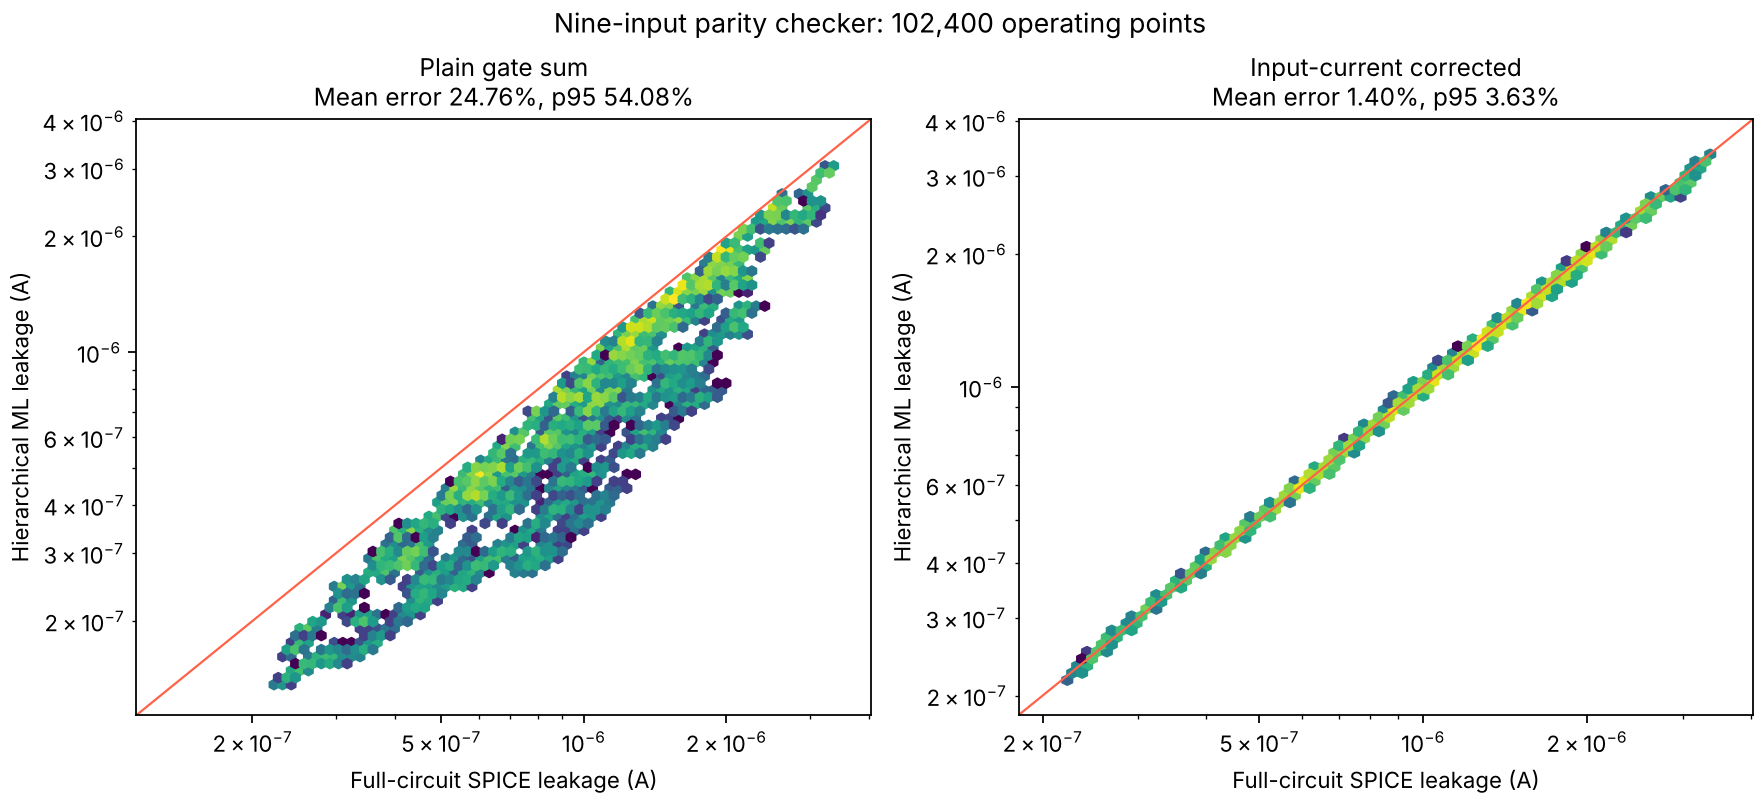
\includegraphics[width=\linewidth]{circuit_parity.png}
\caption{Plain and corrected ML leakage against complete-circuit SPICE
over all 102,400 cases. The diagonal indicates exact agreement.}
\label{fig:circuitparity}
\end{figure}

\begin{figure}[H]
\centering
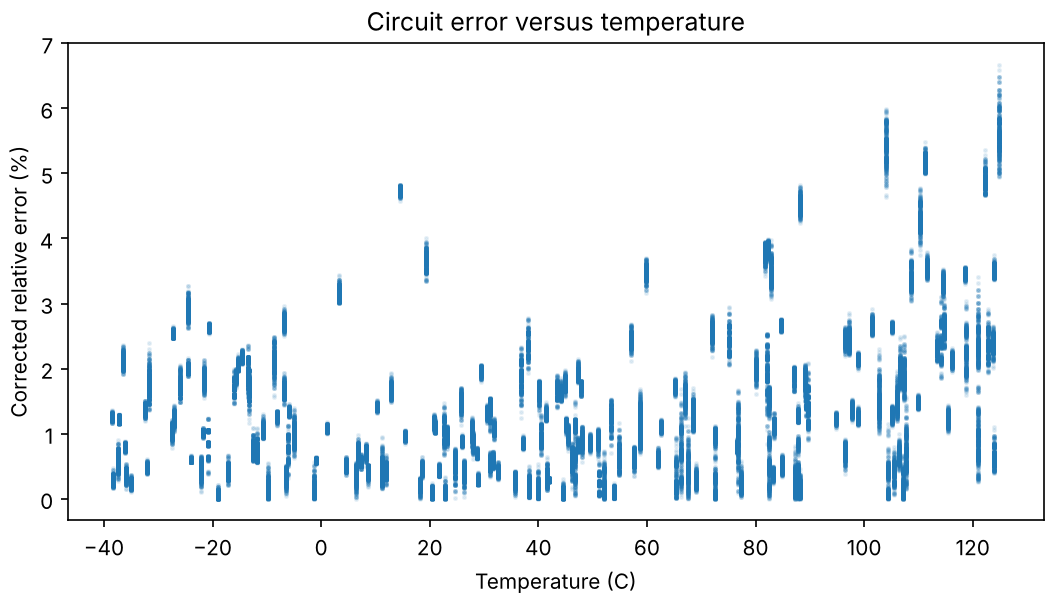
\includegraphics[width=0.85\linewidth]{error_vs_temperature.png}
\caption{Corrected relative error against temperature. Multiple vectors
share each of the 200 PVT corners.}
\label{fig:circuittemperature}
\end{figure}

\subsection{Worked calculation}
For vector \texttt{000000000} at corner 0 ($V_{DD}=0.842208$\,V,
$T=87.773\,^\circ$C), Boolean evaluation gives eight
NAND gates in state \texttt{00}, sixteen in \texttt{01}, none in
\texttt{10}, and eight in \texttt{11}. Thus,
\begin{equation}
\widehat I_{\mathrm{plain}}=
8\widehat I_{00}+16\widehat I_{01}+8\widehat I_{11}.
\end{equation}
The internal high-input currents are then added and the result is compared
with the complete-circuit supply current.
\begin{table}[H]
\centering
\begin{tabular}{lr}
\toprule
Calculation step & Value\\
\midrule
Plain gate sum ($\mu$A) & 1.02026428 \\
Internal high-input correction ($\mu$A) & 0.20789869 \\
Corrected estimate ($\mu$A) & 1.22816297 \\
Complete-circuit SPICE reference ($\mu$A) & 1.24359123 \\
Relative error (\%) & 1.2406 \\
\bottomrule
\end{tabular}
\caption{Worked example for vector \texttt{000000000} at corner 0. The expected parity-error output is 0.}
\end{table}

\subsection{Error analysis and limitations}
The corrected circuit mean error (1.40\%) is lower than the isolated NAND2
mean error (1.79\%; p95 4.56\%). Combining gate contributions can average
some model errors, but the complete circuit also introduces analog loading.
Using exact isolated-gate SPICE currents still gives 0.71\% mean error
after correction, compared with 24.61\% for the uncorrected sum. Thus,
improving transistor fits alone does not remove the error of composing
isolated gates.

The worst individual case is vector \texttt{111111110} at corner 72:
$V_{DD}=0.94936$\,V and $T=124.91\,^\circ$C. SPICE gives
2.92193\,$\mu$A and the corrected model gives 2.72699\,$\mu$A,
an error of 6.67\%. Corner 72 also has the largest mean error over its
512 vectors (5.60\%). Across corners, the worst vector by mean error is
\texttt{111111111}, at 1.49\%.

\begin{table}[H]
\centering
\begin{tabular}{lrr}
\toprule
Temperature range ($^\circ$C) & Mean error (\%) & p95 error (\%)\\
\midrule
$-38.48$ to $6.49$ & 1.24 & 2.71\\
$6.78$ to $44.46$ & 0.97 & 2.36\\
$44.97$ to $84.93$ & 1.28 & 3.56\\
$87.09$ to $124.91$ & 2.13 & 5.14\\
\bottomrule
\end{tabular}
\caption{Corrected error in temperature quartiles, each containing 50
corners and 25,600 cases. Other PVT parameters vary within each group.}
\end{table}

The hottest quartile has the highest mean error, but this is an association
in the sampled corners rather than an isolated causal temperature effect.
With the full-circuit current as the common denominator, mean signed error
splits into $+0.017$ percentage points from ML versus isolated-gate SPICE
and $-0.699$ points from isolated-gate composition versus the full circuit,
giving $-0.682$ points overall. These are signed means, not the median bias.

The lookup assumes ideal input rails and isolated-gate operating points.
In the complete circuit, fanout and departures from ideal high and low
voltages can change leakage. The input-current correction accounts for
internally supplied input currents but does not remove this approximation.
The transistor models also retain prediction errors.

To distinguish these effects, the same aggregation is also evaluated using
isolated-gate SPICE currents in place of ML currents. Its disagreement with
complete-circuit SPICE measures the error of composing isolated gates;
comparison with the ML estimate helps assess the additional model error.
Absolute errors from these comparisons need not add, because signed errors
can cancel.

Possible improvements include gate models conditioned on analog input
voltages and loading, a coupled node-voltage solution, and improved
transistor training coverage. Circuit evaluation cases must remain outside
the training data.

\subsection{Reproducibility and submitted artifacts}
The reported predictions use the regenerated junction-area datasets and
retrained models merged in commit \texttt{29d644c}. The saved full-circuit
SPICE reference already uses the same junction-area convention. The
comparison was refreshed with the new models; retraining is not needed
when reproducing Part 4 from these supplied upstream artifacts.

The command \texttt{python run\_all.py --part4-only} runs the circuit tests,
simulation workflow and comparison. The separate script
\texttt{part4\_circuit/cross\_check.py} runs the operating-point/DC check.
The repository provides the following Part 4 deliverables:
\begin{itemize}
\item Circuit construction, exhaustive logic checks, simulation and
comparison code in \texttt{part4\_circuit/}, with \texttt{run\_all.py}
as the pipeline entry point.
\item Runnable transistor netlists \texttt{parity9\_example.cir} and
\texttt{parity9\_dc.cir} in \texttt{results/part4/}.
\item Compressed full-circuit SPICE records and circuit predictions;
the 800-entry NAND2 lookup; summary tables and both result plots.
\item Per-corner, per-vector and PVT-quartile error tables, worst cases,
and all 32 gate contributions for the worked example.
\item Simulation metadata, package versions and artifact hashes for
tracing the results to their inputs and code.
\end{itemize}
These artifacts retain the baseline and corrected estimates, so the
accuracy improvement and the remaining approximation error can both be
examined directly.
